% Loop Engineering -- A Management Briefing (consulting-style deliverable).
% Self-contained; builds with a standard TeX Live install:  latexmk -pdf loop-engineering-brief.tex
\documentclass[11pt]{article}

\usepackage[T1]{fontenc}
\usepackage[utf8]{inputenc}
\usepackage[scaled=0.95]{helvet}
\renewcommand{\familydefault}{\sfdefault}
\usepackage[table,dvipsnames]{xcolor}
\usepackage[letterpaper,top=0.95in,bottom=1in,left=0.95in,right=0.95in]{geometry}
\usepackage{tikz}
\usetikzlibrary{positioning,arrows.meta,calc}
\usepackage[most]{tcolorbox}
\usepackage{booktabs}
\usepackage{array}
\usepackage{tabularx}
\usepackage{enumitem}
\usepackage{titlesec}
\usepackage{caption}
\usepackage{fancyhdr}
\usepackage[hidelinks]{hyperref}

% ---- palette (consulting navy + bright blue accent) -------------------------
\definecolor{mckdeep}{HTML}{051C2C}
\definecolor{mckblue}{HTML}{2251FF}
\definecolor{mckcyan}{HTML}{00A9F4}
\definecolor{mcksteel}{HTML}{415A6B}
\definecolor{mckgray}{HTML}{6B7B8C}
\definecolor{mcklight}{HTML}{EAF2FB}

% ---- section = action title -------------------------------------------------
\titleformat{\section}{\large\bfseries\color{mckdeep}}{\textcolor{mckblue}{\thesection.}}{0.5em}{}
\titlespacing{\section}{0pt}{14pt}{5pt}
\titleformat{\subsection}{\normalsize\bfseries\color{mcksteel}}{}{0em}{}
\titlespacing{\subsection}{0pt}{8pt}{3pt}

% ---- lists ------------------------------------------------------------------
\setlist[itemize]{leftmargin=1.3em,itemsep=2.5pt,topsep=2pt,parsep=0pt}
\renewcommand{\labelitemi}{\textcolor{mckblue}{\textbf{\textbullet}}}
\setlist[enumerate]{leftmargin=1.5em,itemsep=2.5pt,topsep=2pt,parsep=0pt}

% ---- exhibits ---------------------------------------------------------------
\captionsetup[figure]{name=Exhibit,labelsep=period,font={small},labelfont={bf,color=mckdeep},
  textfont={color=mcksteel}}

% ---- bottom-line callout ----------------------------------------------------
\newtcolorbox{bottomline}{colback=mcklight,boxrule=0pt,sharp corners,
  borderline west={3pt}{0pt}{mckblue},left=10pt,right=8pt,top=5pt,bottom=5pt,
  before skip=6pt,after skip=8pt}

% ---- header / footer --------------------------------------------------------
\pagestyle{fancy}\fancyhf{}
\renewcommand{\headrulewidth}{0pt}
\renewcommand{\footrulewidth}{0.4pt}
\fancyfoot[L]{\footnotesize\color{mckgray}Loop Engineering\,\textbar\,A Management Briefing}
\fancyfoot[R]{\footnotesize\color{mckgray}\thepage}

\newcommand{\sotag}[1]{\textcolor{mckblue}{\textbf{#1}}}

\begin{document}
\thispagestyle{fancy}

% =============================== TITLE =======================================
\noindent{\color{mckblue}\rule{\textwidth}{2.5pt}}
\vspace{4pt}

{\fontsize{24}{27}\selectfont\bfseries\color{mckdeep} Loop Engineering}\\[3pt]
{\large\color{mcksteel} Operating AI coding agents that finish the job ---\\ and how it differs from harness engineering}

\vspace{6pt}
{\footnotesize\color{mckgray} A management briefing \quad\textbar\quad Prepared by Duy Tran Thanh \quad\textbar\quad \texttt{duy.tran10@onemount.com}}
\vspace{2pt}

\noindent{\color{mcklight}\rule{\textwidth}{1.2pt}}

% =============================== EXEC SUMMARY ================================
\begin{tcolorbox}[colback=mckdeep!4,colframe=mckdeep,coltitle=white,
  fonttitle=\bfseries\large,title=Executive summary,sharp corners,boxrule=1pt,
  top=6pt,bottom=6pt,left=8pt,right=8pt]
\begin{itemize}[leftmargin=1.2em,itemsep=4pt,topsep=2pt]
\item \sotag{The shift.} In agentic coding, value has moved from \emph{writing
prompts} to \emph{designing the loop} that runs an agent toward a goal. The
leverage is no longer the single instruction; it is the system that generates
and checks instructions until the work is done.
\item \sotag{The distinction.} \emph{Harness engineering} makes a single step
reliable; \emph{loop engineering} makes a whole goal \emph{finish}, verified and
within a budget. They are complementary, not competing: the loop is one
component of the harness.
\item \sotag{The payoff.} A loop converts a goal into an outcome that is
\emph{trustworthy} (only checked work counts), \emph{auditable} (a full
per-step trail), \emph{cost-bounded} (a hard stop), and \emph{resumable}
(survives interruption). Capable agents run unattended without running away.
\item \sotag{The mandate.} Apply loops where a \emph{human is the bottleneck} on
a repetitive, checkable, multi-step goal --- not where output is merely
unreliable (that is a harness problem). Insist on two non-negotiables: a
built-in check and a hard stop.
\item \sotag{How to start.} Express any task as six plain answers, run a
reference loop in minutes, then scale into CI. A 90-day path is on the last
page.
\end{itemize}
\end{tcolorbox}

% =============================== 1 ===========================================
\section{The bottleneck has moved from model capability to how we operate the model}
\textbf{Situation.} Coding agents are now capable enough to do real, multi-step
engineering work. \textbf{Complication.} Most teams still operate them by hand
--- prompt, read the result, re-prompt --- which caps throughput at human
attention and is error-prone at scale. \textbf{Question.} How do we drive a
capable agent to a finished, trustworthy result \emph{without} a human in every
step?

The answer is to stop hand-steering and instead engineer the \emph{loop}: a
self-running cycle that pursues a goal, checks its own work, remembers progress,
and stops on a defined condition.

\begin{bottomline}
\textbf{Bottom line.} The constraint is no longer ``can the model do it?'' but
``how do we run it to a dependable finish?'' That is an operating-system
question, not a prompting question.
\end{bottomline}

% =============================== 2 ===========================================
\section{Harness and loop engineering solve two different problems --- you need both}
Think of the agent as \emph{model plus harness}, where the harness is everything
around the model. Two disciplines act on it (Exhibit~\ref{ex:overview}):

\begin{itemize}
\item \sotag{Harness engineering} designs the scaffolding for one step ---
context, tools, guardrails, and checks --- so that a single action is reliable.
It asks: \emph{``is this step good?''}
\item \sotag{Loop engineering} designs the cycle that drives the agent across
many steps toward a goal, and owns when to stop. It asks: \emph{``is the whole
goal met, and when do we stop?''}
\end{itemize}

The relationship is precise: the loop is \emph{one component of the harness},
run over time. Harness engineering draws the box; loop engineering animates one
part of it. Exhibit~\ref{ex:compare} contrasts them.

\begin{figure}[t]
\centering
\resizebox{\textwidth}{!}{%
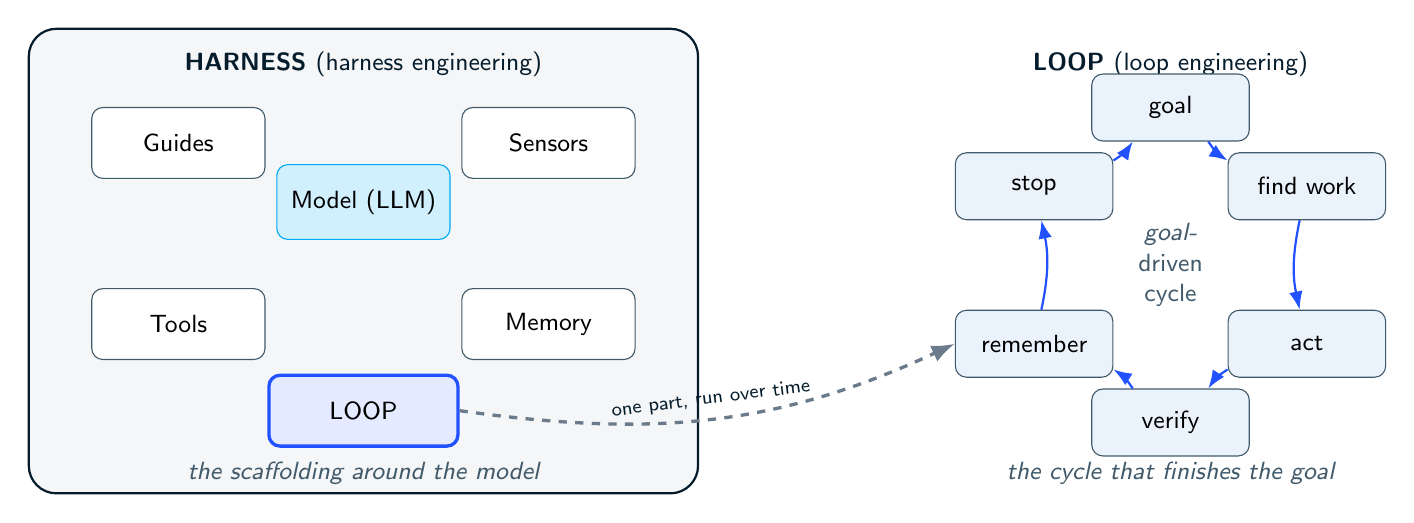
\begin{tikzpicture}[font=\small,>=Latex,
  comp/.style={draw=mcksteel,rounded corners,fill=white,align=center,minimum width=2.2cm,minimum height=0.9cm},
  modeln/.style={draw=mckcyan,fill=mckcyan!18,rounded corners,align=center,minimum width=2.2cm,minimum height=0.95cm},
  loopn/.style={draw=mckblue,very thick,fill=mckblue!12,rounded corners,align=center,minimum width=2.4cm,minimum height=0.9cm},
  ring/.style={draw=mcksteel,fill=mcklight,rounded corners,align=center,minimum width=2.0cm,minimum height=0.85cm}]
% harness
\draw[rounded corners=10pt,fill=mckdeep!4,draw=mckdeep,thick] (-0.5,-3.2) rectangle (8.0,2.7);
\node[color=mckdeep] at (3.75,2.25) {\bfseries HARNESS \textnormal{(harness engineering)}};
\node[modeln] (m) at (3.75,0.5) {Model (LLM)};
\node[comp] (g) at (1.4,1.25) {Guides};
\node[comp] (s) at (6.1,1.25) {Sensors};
\node[comp] (t) at (1.4,-1.05) {Tools};
\node[comp] (mem) at (6.1,-1.05) {Memory};
\node[loopn] (lp) at (3.75,-2.15) {LOOP};
\node[color=mcksteel] at (3.75,-2.95) {\itshape the scaffolding around the model};
% loop ring
\def\cx{14.0}\def\cy{-0.3}
\node[color=mckdeep] at (\cx,2.25) {\bfseries LOOP \textnormal{(loop engineering)}};
\node[ring] (a1) at ($(\cx,\cy)+(90:2.0)$)   {goal};
\node[ring] (a2) at ($(\cx,\cy)+(30:2.0)$)   {find work};
\node[ring] (a3) at ($(\cx,\cy)+(-30:2.0)$)  {act};
\node[ring] (a4) at ($(\cx,\cy)+(-90:2.0)$)  {verify};
\node[ring] (a5) at ($(\cx,\cy)+(-150:2.0)$) {remember};
\node[ring] (a6) at ($(\cx,\cy)+(150:2.0)$)  {stop};
\node[color=mcksteel,align=center] at (\cx,\cy) {\itshape goal-\\driven\\cycle};
\foreach \i/\j in {a1/a2,a2/a3,a3/a4,a4/a5,a5/a6,a6/a1}{\draw[->,thick,mckblue] (\i) to[bend right=12] (\j);}
\node[color=mcksteel] at (\cx,-2.95) {\itshape the cycle that finishes the goal};
\draw[dashed,->,very thick,mckgray] (lp.east) to[out=-8,in=205]
  node[midway,above,sloped,color=mckdeep]{\scriptsize one part, run over time} (a5.west);
\end{tikzpicture}}
\caption{Loop engineering is the part of harness engineering you run over time.
Harness engineering builds everything around the model; the loop is the cycle
that drives it to a finish.}
\label{ex:overview}
\end{figure}

\begin{figure}[t]
\small
\renewcommand{\arraystretch}{1.35}
\rowcolors{2}{mcklight}{white}
\begin{tabularx}{\textwidth}{@{}>{\bfseries\color{mckdeep}}p{0.18\textwidth} >{\raggedright\arraybackslash}X >{\raggedright\arraybackslash}X@{}}
\rowcolor{mckdeep}
\textcolor{white}{Dimension} & \textcolor{white}{\textbf{Harness engineering}} & \textcolor{white}{\textbf{Loop engineering}} \\
What it designs & The scaffolding around the model: context, tools, guardrails, checks & The cycle that drives the agent to a goal \\
Scope          & A single step                                   & A whole run (many steps) \\
Core question  & ``Is this step good?''                          & ``Is the goal met, and when do we stop?'' \\
What it owns   & Reliability of each action                      & Termination and verified completion \\
Input $\rightarrow$ output & Model $+$ context $\rightarrow$ one checked action & Goal $+$ means $\rightarrow$ a verified, auditable, resumable outcome \\
When to invest & Output is unreliable / the agent does the wrong thing & You are the bottleneck on a repetitive, checkable goal \\
\end{tabularx}
\captionof{figure}{The two disciplines are orthogonal: one improves a step, the
other finishes a job. A mature operation invests in both.}
\label{ex:compare}
\end{figure}

\begin{bottomline}
\textbf{Bottom line.} If the symptom is ``wrong output,'' fix the harness. If the
symptom is ``the agent is good but I am stuck driving it,'' build a loop.
\end{bottomline}

% =============================== 3 ===========================================
\section{A loop converts a goal into a verified, auditable, bounded outcome}
A loop is best understood by what goes in and what comes out
(Exhibit~\ref{ex:io}).

\begin{itemize}
\item \sotag{Input --- a goal plus the means to pursue and check it:} the
objective (with a success test), the model, the workspace, any saved progress,
and a verification/termination policy.
\item \sotag{Output --- a terminated, audited outcome:} \emph{why} it stopped;
the completed work, counting \emph{only} items that passed their checks; the
changed files; a replayable per-step trail; and a checkpoint that resumes the
next run.
\end{itemize}

For a decision-maker, the four output properties are the business case:

\begin{itemize}
\item \sotag{Trust} --- only verified work is counted as done.
\item \sotag{Accountability} --- every step leaves an audit trail.
\item \sotag{Cost control} --- a hard budget and stop cap the spend.
\item \sotag{Resilience} --- an interrupted run resumes; nothing is redone.
\end{itemize}

\begin{figure}[t]
\centering
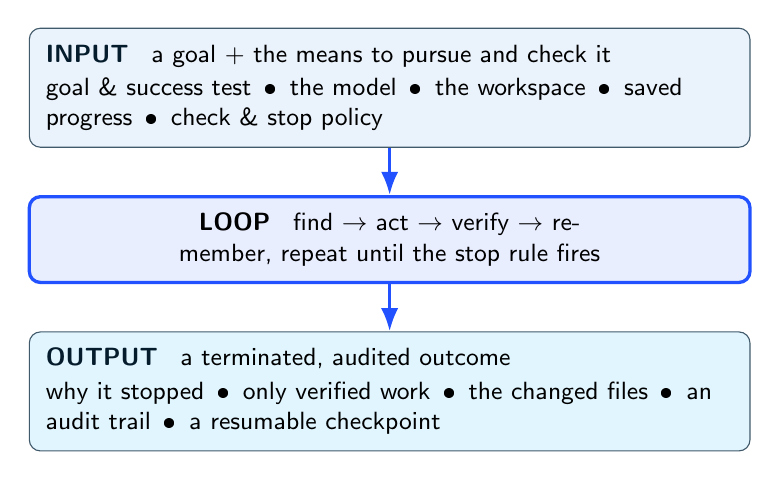
\begin{tikzpicture}[font=\small,>=Latex,node distance=6mm,
  io/.style={draw=mcksteel,rounded corners,align=left,text width=0.72\textwidth,inner sep=6pt},
  mid/.style={draw=mckblue,very thick,rounded corners,fill=mckblue!10,align=center,text width=0.72\textwidth,inner sep=6pt}]
\node[io,fill=mcklight] (in) {\textbf{\color{mckdeep}INPUT}\;\; a goal $+$ the means to pursue and check it\\[1pt]
\small goal \& success test \,\textbullet\, the model \,\textbullet\, the workspace \,\textbullet\, saved progress \,\textbullet\, check \& stop policy};
\node[mid,below=of in] (run) {\textbf{LOOP}\;\; find $\rightarrow$ act $\rightarrow$ verify $\rightarrow$ remember, repeat until the stop rule fires};
\node[io,fill=mckcyan!12,below=of run] (out) {\textbf{\color{mckdeep}OUTPUT}\;\; a terminated, audited outcome\\[1pt]
\small why it stopped \,\textbullet\, only verified work \,\textbullet\, the changed files \,\textbullet\, an audit trail \,\textbullet\, a resumable checkpoint};
\draw[->,very thick,mckblue] (in) -- (run);
\draw[->,very thick,mckblue] (run) -- (out);
\end{tikzpicture}
\caption{What a loop takes in and gives back. The output is trustworthy,
accountable, cost-bounded, and resilient by construction.}
\label{ex:io}
\end{figure}

\begin{bottomline}
\textbf{Bottom line.} A loop is not a faster prompt; it is a managed process that
produces a checkable, accountable result with a known cost ceiling.
\end{bottomline}

% =============================== 4 ===========================================
\section{Apply loops where you are the bottleneck --- not where output is simply unreliable}
The investment decision is a simple triage:
\begin{itemize}
\item Output is unreliable, even on a single step $\rightarrow$ invest in the
\sotag{harness} first (better checks, guides, tools).
\item The agent is reliable per step but the goal is a repetitive, checkable,
multi-step grind that you keep babysitting $\rightarrow$ invest in a \sotag{loop}.
\end{itemize}
Strong first candidates share three traits: a clear ``done'' test, many similar
pieces of work, and low blast-radius per step. Exhibit~\ref{ex:map} lists common
ones.

\begin{figure}[t]
\small
\renewcommand{\arraystretch}{1.35}
\rowcolors{2}{mcklight}{white}
\begin{tabularx}{\textwidth}{@{}>{\bfseries\color{mckdeep}}p{0.22\textwidth} >{\raggedright\arraybackslash}X >{\raggedright\arraybackslash}p{0.22\textwidth} >{\raggedright\arraybackslash}X@{}}
\rowcolor{mckdeep}
\textcolor{white}{Your task} & \textcolor{white}{\textbf{Done when}} & \textcolor{white}{\textbf{One piece of work}} & \textcolor{white}{\textbf{How to check it}} \\
Make tests pass        & the test suite passes            & a failing test       & re-run that test \\
Fix lint / format      & the linter reports zero issues   & a file with warnings & re-run the linter on it \\
Close all TODOs        & no TODO comments remain          & one TODO             & TODO gone, tests still pass \\
Migrate config files   & every file is in the new format  & one old file         & validate against the new schema \\
Upgrade a deprecated API & no calls to the old API remain & one call site        & it still compiles and tests pass \\
\end{tabularx}
\captionof{figure}{Most jobs fit the same shape; you change only three answers
--- what ``done'' means, what one piece of work is, and how to check it.}
\label{ex:map}
\end{figure}

\begin{bottomline}
\textbf{Bottom line.} Loops pay off fastest on repetitive, checkable work where a
human is currently the rate limiter.
\end{bottomline}

% =============================== 5 ===========================================
\section{Implementation: six questions, one spec, runs anywhere}
Turning a task into a loop means answering six plain questions and writing them
in a short spec file:
\begin{enumerate}
\item \textbf{When is it done?} A command that succeeds or a check that comes back clean.
\item \textbf{What are the pieces of work?} How to list what still needs doing.
\item \textbf{How do you do one piece?} Usually: ask the model to fix one thing.
\item \textbf{How do you check it worked?} A test or linter, \emph{wired before the actor.}
\item \textbf{How is progress remembered?} Saved to disk so a restart resumes.
\item \textbf{When should it stop?} Goal met, $N$ tries, or a budget --- always set one.
\end{enumerate}
Questions 1, 4, and 6 are the non-negotiables: a checkable goal, a check before
acting, and a hard stop. The reference framework refuses to run a task that
lacks a check or a stop.

\subsection{The same loop runs in four places}
By changing only \emph{when} it runs and its limit, one loop becomes: a
\sotag{nightly job} (run until nothing new is found); a \sotag{pull-request
gate} (run once; block the merge unless done); a \sotag{bulk migration} (one
file per piece, in isolated copies so parallel work does not clash); or a
\sotag{supervised run} (pause for human approval every few steps).

\begin{bottomline}
\textbf{Bottom line.} The task definition does not change across these surfaces
--- only the trigger and the limit do. Build once, deploy four ways.
\end{bottomline}

% =============================== 6 ===========================================
\section{What to watch for}
Four failure modes account for most trouble; each has a cheap mitigation:
\begin{itemize}
\item \sotag{No way to check ``done.''} The loop cannot tell success from
failure. \emph{Mitigation:} require an explicit check before building the loop.
\item \sotag{Acting before checking.} The agent makes fast, unverified changes.
\emph{Mitigation:} wire the verifier first; count progress only when it passes.
\item \sotag{Unstable work identifiers.} Work repeats after a restart.
\emph{Mitigation:} give each piece a stable name in saved state.
\item \sotag{No stop limit.} The loop runs --- and spends --- forever.
\emph{Mitigation:} a mandatory budget and iteration cap.
\end{itemize}
Governance scales the same way: keep a human on the loop at defined
checkpoints, set token and time budgets, and isolate parallel runs.

\begin{bottomline}
\textbf{Bottom line.} The two failures that cost the most --- no check, no stop ---
are exactly the two the framework blocks before a loop can start.
\end{bottomline}

% =============================== 7 ===========================================
\section{Recommended next steps: a 90-day adoption path}
\begin{enumerate}
\item \sotag{Weeks 1--2 --- Prove the check.} Pick one repetitive, checkable
task. Stand up its automated check (tests or linter). No loop yet.
\item \sotag{Weeks 3--6 --- Run supervised.} Wrap the task in a loop with a hard
stop. Run with a human on the loop. Measure hours saved and ``escape rate''
(bad changes that slipped a check).
\item \sotag{Weeks 7--12 --- Scale into CI.} Promote the loop to a pull-request
gate or nightly job. Add a second task. Set budgets, isolation, and governance
checkpoints.
\end{enumerate}

\begin{tcolorbox}[colback=mckblue!8,colframe=mckblue,coltitle=white,
  fonttitle=\bfseries,title=The one thing to remember,sharp corners,boxrule=1pt]
Treat the loop as a \textbf{managed system} with a goal, a check, and a stop ---
not as a clever prompt. That is what turns a capable agent into dependable,
unattended throughput.
\end{tcolorbox}

\vspace{4pt}
{\footnotesize\color{mckgray} A companion technical report (\texttt{REPORT.md} /
\texttt{loop-engineering.pdf}) provides the formal model, properties, and an
open-source reference implementation (OnLOOP).}

\end{document}
